%!TEX encoding = UTF-8 Unicode

%!TEX root = ../solutions.tex

\ExerciseSolution{\ExeWeekFIVE}


\Task % Uppgift 1

\Subtask 42;\\
 1\\
 2\\
 7\\
 42;\\
 WrappedArray(hej, på, dej)

\Subtask WrappedArray

\Subtask def printAll(xs: Int*) = {println(xs.size); xs.foreach(println)}  

\Subtask Storleken “0” skrivs ut och inget annat.



\Task % Uppgift 2

\Subtask \begin{REPL}
scala.collection.immutable.Vector[IntCell] = 
    Vector([Int](7), [Int](42), [Int](9))
\end{REPL}
Referensena till c2 och xs ändras aldrig. 
xs kommer fortfarande ha tre vektorer som refererar till c1, c2, c3, däremot refererar dessa i sin tur till var sin int som är Mutable. 
I detta fallet ändras c2.x:s referens från 8 till 42.

\Subtask 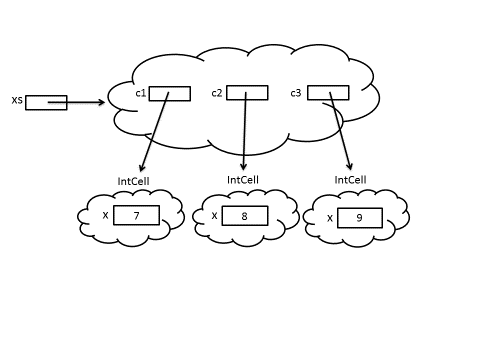
\includegraphics{../img/w05-solutions/memory-pic-1}

\Subtask Istället för att skriva \code{IntCell(var x: Int)} så kan man skriva \code{IntCell(val x: Int)} där varje cells intvärde kommer vara oförändlig. 
Alltså då attributen till objekten är “Val” så kommer även de att vara oförändliga. 


\Task % Uppgift 3

\Subtask \begin{Code}
def copyAppend(xs: Array[Int], x: Int): Array[Int] = {
  val n = xs.size
  val ys = Array[Int](n+1)
  var i = 0
  while(i < n) {
    ys(i) = xs(i)
    i += 1	
  }
  ys(n) = x
  ys
}
\end{Code}

\Subtask \begin{REPL}
xs: scala.collection.mutable.ArrayBuffer[Int] = ArrayBuffer()
ArrayBuffer(1, 1, 2)
ArrayBuffer(1, 1, 2, 3)
ArrayBuffer(1, 1, 2, 3, 5)
ArrayBuffer(1, 1, 2, 3, 5, 8)
ArrayBuffer(1, 1, 2, 3, 5, 8, 13)
ArrayBuffer(1, 1, 2, 3, 5, 8, 13, 21)
ArrayBuffer(1, 1, 2, 3, 5, 8, 13, 21, 34)
ArrayBuffer(1, 1, 2, 3, 5, 8, 13, 21, 34, 55)
ArrayBuffer(1, 1, 2, 3, 5, 8, 13, 21, 34, 55, 89)
ArrayBuffer(1, 1, 2, 3, 5, 8, 13, 21, 34, 55, 89, 144)
Int = 144
Int = 12
\end{REPL}

\Subtask \code{xs.size = 46}\\
\code{xs(45) = 1836311903}\\
(Ha en arrayBuffer av typen Long istället och byt 100 mot Int.MaxValue och ta det nästsista elementet i sekvensens (det sista kommer vara över)) 

\Task % Uppgift 4

\Subtask Nej det gör det inte. 
Då ys tilldelas xs.toArray kopieras datan från xs över i en array (som är mutable) vilket är en annan referens än den till xs. 
Detta innebär att xs och ys inte “pekar” på samma objekt längre.

\Subtask Ja därför båda är array och nu kopieras referensen till ys över till zs. 
Därför kommer alla ändringar i zs att påverka ys (så länge de pekar på samma referens).

\Subtask Nej det gör det inte. Se a).


\Task % Uppgift 5

\Subtask Den andra parametern anger hur stor den nya vektorn som returneras ska vara.

\Subtask \begin{enumerate}
\item 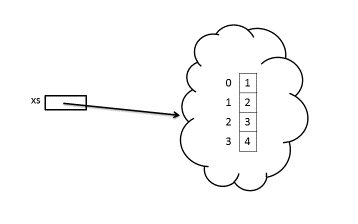
\includegraphics[scale=1.2]{../img/w05-solutions/memory-pic-2}
\item 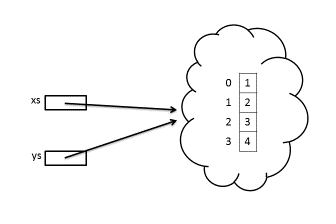
\includegraphics[scale=1.2]{../img/w05-solutions/memory-pic-3}
\item 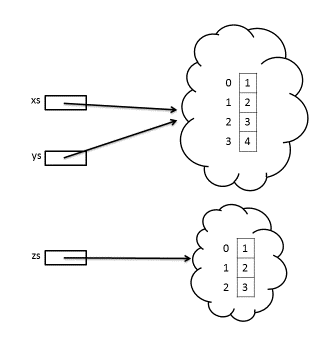
\includegraphics[scale=1.2]{../img/w05-solutions/memory-pic-4}
\item 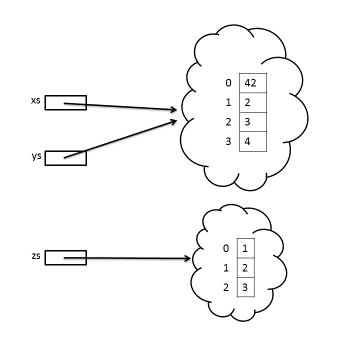
\includegraphics[scale=1.2]{../img/w05-solutions/memory-pic-5}
\item 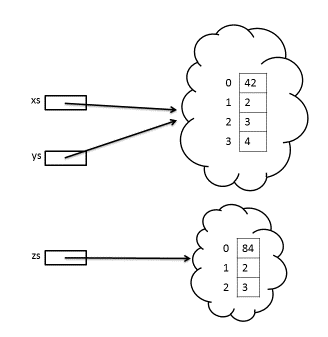
\includegraphics[scale=1.2]{../img/w05-solutions/memory-pic-6}
\end{enumerate}
xs = Array(42, 2, 3, 4)\\
ys = Array(42, 2, 3 ,4)\\
zs = Array(84, 2, 3)\\
\code{xs} och \code{yx} refererar till samma objekt och då deras första IntCell:s värde ändras till 42, så kommer förändringen att ske för båda.
\code{zs} har en referens till ett annat objekt med ett mindre element. Att \code{zs}:s första element ändras, påverkar inte \code{xs} och \code{ys}.


\Task % Uppgift 6

\Subtask \begin{Code}
def seqReverseCopy(xs: Array[Int]): Array[Int] = {
  val n = xs.size
  val ys = Array[Int](n)
  var i = 0
  while(i < n) {
    ys(n-i-1) = xs(i)
    i += 1
  }
  ys
}
\end{Code}

\Subtask \begin{Code}
def seqReverseCopy(xs: Array[Int]): Array[Int] = {
  val n = xs.size
  val ys = Array[Int](n)
  for(i <- n-1 to 0 by -1) ys(n-i-1) = xs(i)
  ys
}
\end{Code}

\Subtask Se b).


\Task % Uppgift 7

\Subtask \begin{Code}
def reverseString(s: String): String = {
  val sb = new StringBuilder(s)
  val n = sb.length
  for (i <- 0 until n / 2) { 
    val temp = sb(i)
    sb(i) = sb(n - i - 1)
    sb(n - i - 1) = temp
  }
  sb.toString     
}
\end{Code}

\Subtask \begin{Code}
def isPalindrome(s: String): Boolean = {s == reverseString(s)}
\end{Code}

\Subtask \begin{Code}
def isPalindrome(s: String): Boolean = {
  val n = s.length
  var foundDiff = false
  var i = 0
  while (i < n/2 && !foundDiff)  { 
    foundDiff = s(i) != s(n - i - 1)
    i += 1
  }
  !foundDiff
}
\end{Code}


\Task % Uppgift 8

\Subtask \code{xs.filter(_ == 6).size}

\Subtask \code{xs.filter(_ % 2 == 0).size}

\Subtask \begin{REPL}
scala.collection.immutable.Map[Int,scala.collection.immutable.Vector[Int]] = 
	Map(1 -> Vector(5, 3, 1, 1, 3, 5, 1, 1, 3), 0 -> Vector(6, 6, 2, 6))
scala.collection.immutable.Map[Int,scala.collection.immutable.Vector[Int]] = 
	Map(1 -> Vector(5, 3, 1, 1, 3, 5, 1, 1, 3), 0 -> Vector(6, 6, 2, 6))
scala.collection.immutable.Map[Int,scala.collection.immutable.Vector[Int]] = 
	Map(2 -> Vector(5, 5, 2), 1 -> Vector(1, 1, 1, 1), 0 -> Vector(3, 6, 3, 6, 3, 6))
(2,Vector(5, 5, 2))
(1,Vector(1, 1, 1, 1))
(0,Vector(3, 6, 3, 6, 3, 6))
freqEvenOdd: scala.collection.immutable.Map[Int,Int] = Map(1 -> 9, 0 -> 4)
nEven: Int = 4
nOdd: Int = 9
\end{REPL}

\Subtask \code{xs.groupBy(i => i)} skapar en map där nycklarna är alla unika element och värdena är av samma värde som respektive nyckel. 

\Subtask \code{val freq: Map[Int, Int] = xs.groupBy(i => i).map(p => (p._1, p._2.size))}

\Subtask \begin{Code}
def tärningsRegistrering(xs: Array[Int]): Array[Int] = {
  val f = Array.fill(7)(0)
  f(0) = xs.size
  var i = 0
  while (i < f(0)) {
    f(xs(i)) += 1
    i += 1
  }
  f 
}
\end{Code}


\Task % Uppgift 9

\Subtask  

\begin{algorithm}[H]
 \SetKwInOut{Input}{Indata}\SetKwInOut{Output}{Resultat}
 
 \Input{En sekvens $xs$ av typen \texttt{Array[Int]} och $pos$}
 \Output{En ny sekvens av typen \texttt{Array[Int]} som är en kopia av $xs$ fast med elementet på plats $pos$ borttaget}
 $n \leftarrow$ antalet element $xs$\\ 
 $ys \leftarrow$ en ny \texttt{Array[Int]} med plats för $n-1$ element \\
 \For{$i \leftarrow 0$ \KwTo $pos - 1$}{
  $ys(i) \leftarrow xs(i)$
 }
 $ys(pos) \leftarrow x$ \\
 \For{$i \leftarrow pos+1$ \KwTo $n - 1$}{
  $ys(i - 1) \leftarrow xs(i)$
 }
 \Return $ys$ 
\end{algorithm}

\Subtask \begin{Code}
def removeCopy(xs: Array[Int], pos: Int): Array[Int] = {
  val n = xs.size
  val ys = Array.fill(n - 1)(0)
  for (i <- 0 until pos) ys(i) = xs(i)
  for (i <- pos+1 until n) ys(i - 1) = xs(i)
  ys
} 
\end{Code}


\Task % Uppgift 10

\Subtask  

\begin{algorithm}[H]
 \SetKwInOut{Input}{Indata}\SetKwInOut{Output}{Resultat}
 
 \Input{En sekvens $xs$ av typen \texttt{Array[Int]} och $pos$}
 \Output{En uppdaterad sekvens av $xs$ där elementet på plats $pos$ tagits bort och efterföljande element flyttas ett steg mot lägre index med ett sista elementet som är $0$}
 $n \leftarrow$ antalet element $xs$\\ 
 \For{$i \leftarrow pos+1$ \KwTo $n - 1$}{
  $xs(i - 1) \leftarrow xs(i)$
 }
 $xs(n - 1) \leftarrow 0$ \\
\end{algorithm}

\Subtask \begin{Code}
def remove(xs: Array[Int], pos: Int): Unit = {
  val n = xs.size
  for (i <- pos+1 until n) xs(i - 1) = xs(i)
  xs(n-1) = 0
} 
\end{Code}


\Task % Uppgift 11

\Subtask Antingen kan du skapa en ny instans av \code{java.util.Random} genom att skriva: \code{val r1 = new java.util.Random}. 
Men om \code{java.util.Random} importeras kan “java.util” skippas och istället skrivs: \code{val r2 = new Random}. 
Som valfritt argument kan ett slumptalsfrö av typen Long skickas med när en ny instans skapas, e.g. \code{val r3 = new Random(42L)}.
\code{nextInt(x)} skapar ett slumptal från och med 0, upp till x (exklusive x).

\Subtask \begin{REPL}
import java.util.Random // Importerar Random

frö: Long = 42 // Ett slumptalsfrö av värdet 42L skapas.

  // Skapar ett Random objekt med slumptalsfrö "frö".
rnd: java.util.Random = java.util.Random@2f410acf 

res0: Int = 7 // Slumpade fram ett tal från 0 till och med 9.

9 8 8 8 9 7 2 1 4 0 0 3 8 8 4 5 9 1 3 3 5 1 1 
3 3 3 6 3 4 7 5 7 8 7 6 9 7 0 3 0 6 6 1 0 8 1 
1 1 0 5 3 5 1 5 3 5 9 9 5 1 8 9 0 6 4 7 5 7 9 
6 4 0 8 1 0 9 6 6 3 2 7 9 2 7 0 6 9 8 5 0 0 8 
9 2 7 7 3 5 1 3 // Slumpar och skriver ut 100 tal från 0 till och med 9.

  // Skapar ett Random objekt med slumptalsfrö "frö". 
rnd1: java.util.Random = java.util.Random@31e4bb20 

  // Skapar ett Random objekt med slumptalsfrö "frö".
rnd2: java.util.Random = java.util.Random@45e37a7e 

  // Skapar ett Random objekt med slumptalsfrö med 
  // värdet av vad tiden är just nu i nanosekunder.
rnd3: java.util.Random = java.util.Random@57eda880 

  // Skapar ett Random objekt med slumptalsfrö 
  // med värdet (math.random * Long.MaxValue).toLong.
rnd4: java.util.Random = java.util.Random@79da1ec0 

flip: (r: java.util.Random)String // Skapar en funktion som singlar slant.

  // Singlar slant med alla fyra Random 
  // objekt 100 gånger samt printar ut resultatet.
xs: scala.collection.immutable.IndexedSeq[(String, String, String, String)] = 
Vector((krona,krona,krona,klave), (klave,klave,krona,krona), (krona,krona,klave,klave), 
(klave,klave,krona,klave), (klave,klave,krona,krona), (krona,krona,klave,krona), 
(klave,klave,klave,klave), (krona,krona,klave,krona), (krona,krona,klave,krona), 
(klave,klave,krona,klave), (krona,krona,krona,klave), (klave,klave,krona,klave), 
(klave,klave,krona,krona), (klave,klave,klave,krona), (klave,klave,klave,krona), 
(krona,krona,klave,klave), (klave,klave,klave,klave), (krona,krona,klave,krona), 
(krona,krona,klave,klave), (krona,krona,klave,klave), (krona,krona,klave,krona), 
(klave,klave,klave,klave), (klave,klave,krona,krona), (klave,klave,klave,klave), 
(krona,krona,krona,krona), (krona,krona,krona,klave)... 

  // Kollar om det finns något värde som rnd1
  // har genererat men som inte rnd2 genererat.
res1: Boolean = false 

  // Kollar om det finns något värde som rnd1
  // har genererat men som inte rnd3 genererat.
res2: Boolean = true 

\end{REPL}

\Subtask Vid felsökning och vid simulering där man vill att samma “slumpmässiga” sekvens uppstår varenda gång.

\Subtask Ja.

\Subtask \url{https://docs.oracle.com/javase/7/docs/api/java/lang/Math.html#random%28%29--} säger att den skapar ett nytt java.util.Random-objekt.

\Subtask Den skapar ett slumpmässigt slumptalsfrö. För mer information, se: \url{https://docs.oracle.com/javase/8/docs/api/java/util/Random.html#Random--}


\Task % Uppgift 12

\begin{Code}
def testRandom(r: Random, n: Int): Unit = {
  val xs = Array.fill(n)(r.nextInt(6) + 1)
  val f = tärningsRegistrering(xs)
  println("Antal kast: " + f(0))
  for (i <- 1 to 6) println(s"Antal $i:or: " + f(i)) 
}
\end{Code}


\Task % Uppgift 13

\Subtask -

\Subtask \begin{REPL}
Rolling the dice 10000 times with seed 42
Number of 1's: 1654
Number of 2's: 1715
Number of 3's: 1677
Number of 4's: 1629
Number of 5's: 1643
Number of 6's: 1682
\end{REPL}
Simulerar 10000 tärningskast (med slumptalsfrö 42) och skriver ut förekomsten av respektive tärningskast.

\Subtask Array i scala deklararas: \code{val scalaArray = Array.ofDim[Int](6)} medan i java skrivs: \code{int[] javaArray = new int[6];}
\code{for}-sats i scala skrivs: \code{for(i <- 0 to n)} medan i java skrivs: \code{for (int i = 0; i < n; i++)}. 
I java måste semicolon skrivas efter varje operation samt att typen måste explicit definieras vid variabeldeklaration. 
I scala behövs inga semicolon (förutom för att separera operationer på samma rad) och scala bestäms typen implicit, alltså att kompilatorn “gissar” typen av variabeln som deklareras.

\Subtask Lägg till \code{System.out.println(i);} i for-looparna

\Subtask \begin{Code}[language=Java] 
// DiceReg2.java
import java.util.Random;
public class DiceReg2{
	public static int[] diceReg = new int[6];
	private static Random rnd = new Random();
	
	public static int parseArguments(String[] args){
		int n = 100;
		if(args.length > 0) {
			n = Integer.parseInt(args[0]);
		}
		if(args.length > 1) {
			int seed = Integer.parseInt(args[1]);
			rnd.setSeed(seed);
		}
		return n;
	}
	
	public static void registerPips(int n) {
		for(int i = 0; i<n; i++) {
			int pips = rnd.nextInt(6);
			diceReg[pips]++;
		}
	}
	
	public static void main(String[] args) {
		int n = parseArguments(args);
		registerPips(n);
		printReg();
	}
}
\end{Code}

\Subtask \begin{REPL} 
  // Skriver ut förekomsten av 1000 tärningskast med slumptalsfrö 42.
Number of 1's: 165
Number of 2's: 163
Number of 3's: 178
Number of 4's: 183
Number of 5's: 156
Number of 6's: 155

  // Skriver ut diceReg-attributet
res1: Array[Int] = Array(165, 163, 178, 183, 156, 155)

  // Skriver ut diceReg-attributet efter 1000 till kast.
res2: Array[Int] = Array(329, 325, 349, 360, 324, 313)

  // Skriver ut diceReg-attributet efter 1000 till kast.
res3: Array[Int] = Array(498, 484, 531, 513, 485, 489)

  // Det blir runtime error då attributet rnd är 
  // private och kan inte nås via REPL:n.
<console>:11: error: value rnd is not a member of object DiceReg2
	DiceReg2.rnd
				    ^
\end{REPL}

\Subtask \begin{REPL}
value [diceReg/rnd] is not a member of object DiceReg2
\end{REPL}

\Subtask Om man ska spara under någon data som man inte vill att användaren, eller någon annan, inte ska kunna komma åt. 
T.ex. om du gör en bankapp vill du inte att nyckeln som du använder för att autorisera en användare ska vara tillgänglig för då kan hackare använda det för att ta sig in på kontot och stjäla pengar!


\Task % Uppgift 14

\Subtask \code{hasNextInt()} kollar enbart om det finns ett till tal och returnerar \code{true}/\code{false}. \code{nextInt()} “hoppar” till nästa tal och returnerar det.
Se \url{https://docs.oracle.com/javase/7/docs/api/java/util/Scanner.html#hasNextInt%28%29} och \url{https://docs.oracle.com/javase/7/docs/api/java/util/Scanner.html#nextInt%28%29 }.

\Subtask -

\Subtask -

\Subtask \begin{Code}[language=Java,numbers=left]
import java.util.Random;
import java.util.Scanner;

public class DiceScanBuggy {
	public static int[] diceReg = new int[6];
	public static Scanner scan = new Scanner(System.in);
	
	public static void registerPips() {
		System.out.println("Enter pips separated by blanks: ");
		System.out.println("End with -1 and <Enter>.");
		boolean isPips = true;
		while(isPips && scan.hasNextInt()){
			int pips = scan.nextInt();
			if(pips >= 1 && pips <= 6) {
				diceReg[pips-1]++;
			} else {
				isPips = false;
			}
		}
	}
  
	public static void printReg(){
		for(int i = 1; i<7; i++) {
		System.out.println("Number of " + i + "'s: " + diceReg[i-1]);
		}
	}
  
	public static void main(String[] args) {
		registerPips();
		printReg();
	}
}
\end{Code}

\Task % Uppgift 15

\Subtask \code{ArrayBuffer}.

\Subtask \code{ArrayBuffer} eller \code{Array}.

\Subtask \code{Array}.

\Subtask \code{Vector}.



\ExtraTasks %%%%%%%%%%%%

\Task % Uppgift 16

\Subtask \begin{Code}
def insertCopy(xs: Array[Int], x: Int, pos: Int): Array[Int] = {
  val n = xs.size
  val ys = Array.ofDim[Int](n + 1)
  for (i <- 0 until pos) ys(i) = xs(i)
  ys(pos) = x
  for (i <- pos until n) ys(i + 1) = xs(i)
  ys
} 
\end{Code}

\Subtask \code{pos} måste vara \code{0}.

\Subtask \begin{REPL}
java.lang.ArrayIndexOutOfBoundsException: -1
\end{REPL}

\Subtask Elementet \code{x} läggs till på slutet av arrayen, alltså kommer den returnerande arrayen vara större än den som skickades in.

\Subtask \begin{REPL}
java.lang.ArrayIndexOutOfBoundsException: 5
\end{REPL}
Man får \code{ArrayIndexOutOfBoundsException} då indexeringen är utanför storleken hos arrayen.

\Task % Uppgift 17

\Subtask 

\begin{algorithm}[H]
 \SetKwInOut{Input}{Indata}\SetKwInOut{Output}{Resultat}
 
 \Input{En sekvens $xs$ av typen \texttt{Array[Int]} och heltalen $x$ och $pos$}
 \Output{En uppdaterad sekvens av $xs$ där elementet $x$ har satts in på platsen $pos$ och efterföljande element flyttas ett steg där sista elementet försvinner}
 $n \leftarrow$ antalet element $xs$\\ 
 $ys \leftarrow$ en klon av $xs$\\
 $xs(pos) \leftarrow x$\\ 
 \For{$i \leftarrow pos+1$ \KwTo $n - 1$}{
  $xs(i) \leftarrow ys(i - 1)$
 }
\end{algorithm}

\Subtask \begin{Code}
def insert(xs: Array[Int], x: Int, pos: Int): Unit = {
  val n = xs.size
  val ys = xs.clone
  xs(pos) = x
  for (i <- pos + 1 until n) xs(i) = ys(i - 1)
} 
\end{Code}


\Task % Uppgift 18

\begin{Code}
def tärningsRegistrering(xs: Array[Int]): Array[Int] = {
  val f = Array.fill(7)(0)
  f(0) = xs.size
  for(i <- 0 until f(0)) f(xs(i)) += 1
  f 
}
\end{Code}


\Task % Uppgift 19



\AdvancedTasks %%%%%%%%%


\Task % Uppgift 20

\Subtask

\Subtask


\Task % Uppgift 21

\Subtask

\Subtask

\Subtask


\Task % Uppgift 22


\Task % Uppgift 23

\Subtask

\Subtask

\Subtask